% Thick cylinder under internal pressure (Rajendran 2010, Sect. 5.9; code:
% studies/thick_cylinder/matlab): (a) quarter annulus 1 <= r <= 3, internal
% pressure p_i = 1000 on r = 1, r = 3 traction-free, symmetry conditions
% u_x = 0 on x = 0 and u_y = 0 on y = 0 (cyl_solve.m, Lame problem),
% E = 1000, nu = 0.25, plane stress (run_study.m); (b) one super-element of
% 2 x 2 elements: the four interior mid-side nodes (open circles) are rotated
% counter-clockwise by alpha about the centre node (filled dots, schematic,
% alpha = 30 deg); (c)-(h) meshes for N = 2 (4 x 4 elements).
% data: cyl_mesh_N2_a<alpha>.dat
\tracinglostchars=0 % blank lines (jumps) in the mesh data
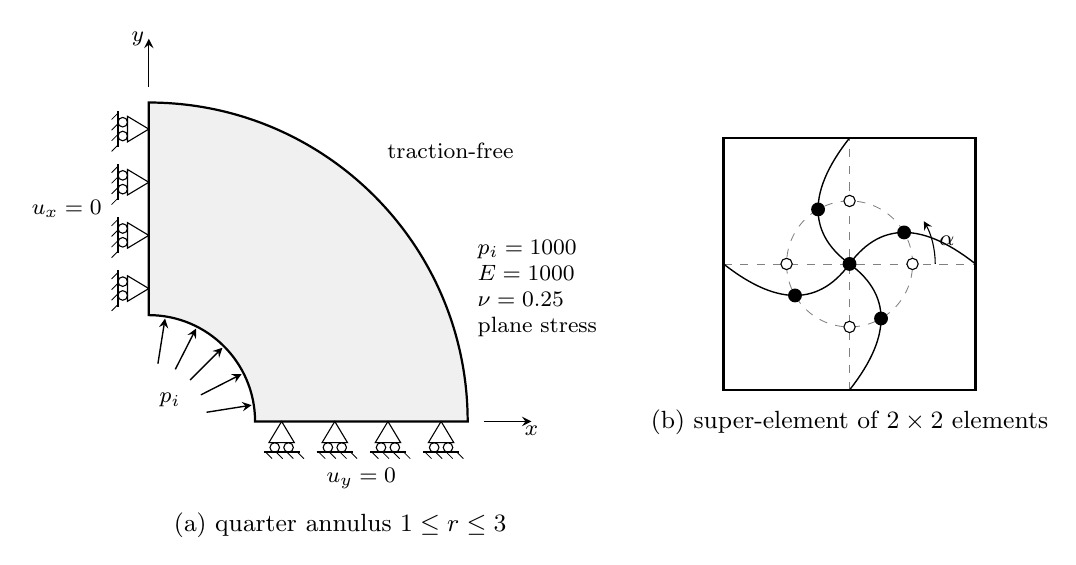
\begin{tikzpicture}[x=1.35cm, y=1.35cm,
    plabel/.style={anchor=north, font=\small, inner sep=0pt, align=center},
    slabel/.style={font=\footnotesize, inner sep=1.5pt},
    body/.style={draw=black, fill=gray!12, line width=0.8pt},
    roller/.pic={% apex at the node, restrains the displacement in the pic's x direction
      \draw[line width=0.4pt, fill=white] (0,0) -- (-0.2,0.12) -- (-0.2,-0.12) -- cycle;
      \draw[line width=0.4pt] (-0.245,0.065) circle (0.045) (-0.245,-0.065) circle (0.045);
      \draw[line width=0.6pt] (-0.29,0.17) -- (-0.29,-0.17);
      \foreach \s in {-0.15,-0.05,0.05,0.15} \draw[line width=0.3pt] (-0.29,\s) -- (-0.35,\s-0.06);}]
% (a) problem
\begin{scope}
  \draw[body] (1,0) -- (3,0) arc[start angle=0, end angle=90, radius=3] -- (0,1)
    arc[start angle=90, end angle=0, radius=1] -- cycle;
  \foreach \t in {9,27,...,81}
    \draw[-stealth, line width=0.5pt] ({0.55*cos(\t)},{0.55*sin(\t)}) -- ({0.98*cos(\t)},{0.98*sin(\t)});
  \node[slabel] at (0.2,0.2) {$p_i$};
  \foreach \s in {1.25,1.75,2.25,2.75} {
    \pic at (0,\s) {roller};
    \pic[rotate=90] at (\s,0) {roller};}
  \node[slabel, anchor=east] at (-0.4,2) {$u_x=0$};
  \node[slabel, anchor=north] at (2,-0.4) {$u_y=0$};
  \draw[-stealth, line width=0.5pt] (3.15,0) -- (3.6,0) node[slabel, below] {$x$};
  \draw[-stealth, line width=0.5pt] (0,3.15) -- (0,3.6) node[slabel, left] {$y$};
  \node[slabel, anchor=west, align=left] at (2.2,2.55) {traction-free};
  \node[slabel, align=left, anchor=west] at (3.05,1.25)
    {$p_i=1000$\\$E=1000$\\$\nu=0.25$\\plane stress};
  \node[plabel] at (1.8,-0.85) {(a) quarter annulus $1\le r\le3$};
\end{scope}
% (b) super-element: interior mid-side nodes rotated by alpha (schematic)
\begin{scope}[xshift=8.9cm, yshift=2.0cm, x=1.6cm, y=1.6cm]
  \draw[gray, dashed, line width=0.3pt] (-1,0) -- (1,0) (0,-1) -- (0,1);
  \draw[gray, dashed, line width=0.3pt] (0,0) circle (0.5);
  \foreach \k in {0,90,180,270}
    \draw[black, line width=0.5pt] plot[domain=-1:1, samples=31, variable=\s]
      ({0.5*cos(\k+30)*(1-\s*\s) + cos(\k)*\s*(\s+1)/2},
       {0.5*sin(\k+30)*(1-\s*\s) + sin(\k)*\s*(\s+1)/2});
  \draw[line width=0.8pt] (-1,-1) rectangle (1,1);
  \foreach \k in {0,90,180,270} {
    \draw[fill=white, line width=0.4pt] ({0.5*cos(\k)},{0.5*sin(\k)}) circle (0.045);
    \fill ({0.5*cos(\k+30)},{0.5*sin(\k+30)}) circle (0.055);}
  \fill (0,0) circle (0.055);
  \draw[-stealth, line width=0.4pt] (0.68,0) arc[start angle=0, end angle=30, radius=0.68];
  \node[slabel, anchor=west] at ({0.7*cos(15)},{0.7*sin(15)}) {$\alpha$};
  \node[plabel] at (0,-1.15) {(b) super-element of $2\times2$ elements};
\end{scope}
\end{tikzpicture}\par\bigskip
\begin{tikzpicture}[plabel/.style={anchor=north, font=\small, inner sep=0pt}]
\begin{groupplot}[group style={group size=3 by 2, horizontal sep=0.9cm, vertical sep=0.85cm},
    hide axis, clip=false, x=1.62cm, y=1.62cm, xmin=0, xmax=3, ymin=0, ymax=3,
    mesh/.style={black, line width=0.4pt}]
  \nextgroupplot
    \addplot[mesh] table {\data/cyl_mesh_N2_a000.dat};
    \node[plabel] at (axis cs:1.5,-0.1) {(c) $\alpha=0^\circ$};
  \nextgroupplot
    \addplot[mesh] table {\data/cyl_mesh_N2_a015.dat};
    \node[plabel] at (axis cs:1.5,-0.1) {(d) $\alpha=15^\circ$};
  \nextgroupplot
    \addplot[mesh] table {\data/cyl_mesh_N2_a030.dat};
    \node[plabel] at (axis cs:1.5,-0.1) {(e) $\alpha=30^\circ$};
  \nextgroupplot
    \addplot[mesh] table {\data/cyl_mesh_N2_a045.dat};
    \node[plabel] at (axis cs:1.5,-0.1) {(f) $\alpha=45^\circ$};
  \nextgroupplot
    \addplot[mesh] table {\data/cyl_mesh_N2_a060.dat};
    \node[plabel] at (axis cs:1.5,-0.1) {(g) $\alpha=60^\circ$};
  \nextgroupplot
    \addplot[mesh] table {\data/cyl_mesh_N2_a090.dat};
    \node[plabel] at (axis cs:1.5,-0.1) {(h) $\alpha=90^\circ$};
\end{groupplot}
\end{tikzpicture}
